\chapter{Исследовательская часть}

\section{Технические характеристики}

Ниже приведены технические характеристики устройства, на котором выполнялось тестирование.

\begin{itemize}
	\item Операционная система: macOS 14.6.1.
	\item Объём оперативной памяти: 18 Гб.
	\item Процессор: Apple M3 Pro.
\end{itemize}

Тестирование проводилось на ноутбуке, включённом в сеть электропитания. Во время тестирования ноутбук был нагружен только встроенными приложениями окружения, а также непосредственно системой тестирования.

% 

\section{Время выполнения реализаций алгоритмов}

Алгоритмы тестировались с помощью запуска утилит тестирования программ на языке Golang \cite{testing_functions} \cite{testing_flags} \cite{pprof}. Данные утилиты запускают бенчмарк для функции, реализующей нечёткий логический вывод, и замеряют процессорное время её выполнения \cite{golang_prof}. Среднее время выполнения одного вывода составило 19.971 мс. На рисунке \ref{img:deviation} приведены график зависимости среднеквадратичного отклонения расстояния (СКО) между лидером и автопилотом от скорости лидера. Эталонное расстояние между лидером и автопилотом было равно 15 метрам.

\begin{figure}[h!]
	\begin{center}
		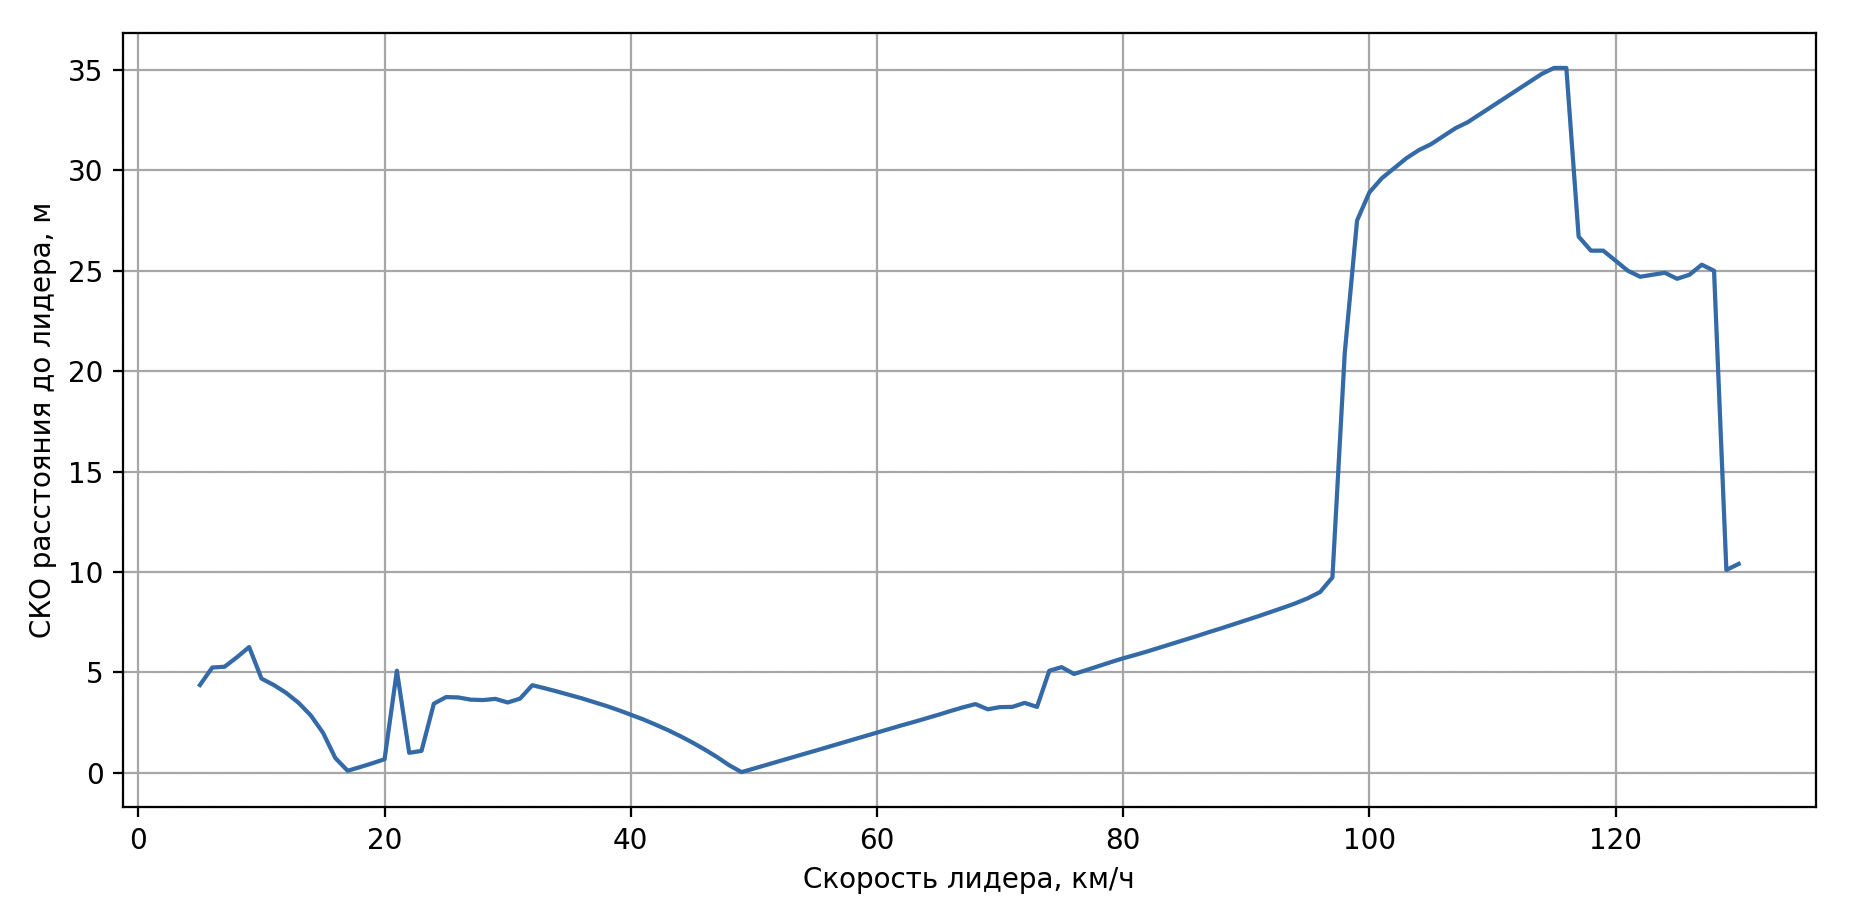
\includegraphics[width=\textwidth]{images/deviation.png}
	\end{center}
	\caption{График зависимости СКО расстояния между лидером и автопилотом от скорости лидера}
	\label{img:deviation}
\end{figure}

\section*{Вывод}

В данном разделе были приведены результаты замеров времени вычисления скорости автопилота и среднеквадратичной ошибки расстояния между лидером и автопилотом. Время выполнения одного нечёткого логического вывода в среднем составило 19.971 мс. Минимальное значение среднеквадратичного отклонения расстояния между лидером и автопилотом составило 0.1 м, максимальное --- 35.1 м. Для повышения точности реализованной нечёткой модели необходимо либо переработать базу правил, дополнив её новыми правилами или изменив существующие, либо увеличить число нечётких переменных.

\clearpage
